\documentclass{beamer}
% Setup for bibliography
\usepackage[
backend=biber,
style=numeric-comp,
]{biblatex}
\addbibresource{../../references.bib}

% Pretty self explanatory
% We sue this in title bits
\usepackage{datetime}

% Standard math packages / setup
\usepackage{amsmath} 
\usepackage{amsfonts}
\usepackage{amsthm}
\usepackage{amssymb} 
\usepackage{accents}
\usepackage{mathrsfs}
\usepackage{mathtools}

\usepackage{bm}

%\newtheorem{lemma}{Lemma}
%\newtheorem{theorem}{Theorem}
%\newtheorem{definition}{Definition}

% So we can import pngs
\usepackage{graphicx} 

% This gives us nice clickable links 
% https://www.overleaf.com/learn/latex/Hyperlinks#Styles_and_colours
\usepackage{hyperref}
\hypersetup{
    colorlinks=true,
    linkcolor=blue,
    citecolor=blue,
    filecolor=magenta,      
    urlcolor=cyan,
    pdftitle={Monte Carlo Methods (DRAFT)},
    pdfpagemode=FullScreen,
    }
\urlstyle{same}

% Allows us to define colors
% We use this in the next block, listings
\usepackage{color}
\definecolor{dkgreen}{rgb}{0,0.6,0}
\definecolor{gray}{rgb}{0.5,0.5,0.5}
\definecolor{mauve}{rgb}{0.58,0,0.82}

% Allows us to include 
\usepackage{listings}
\lstset{frame=tb,
  language={},
  aboveskip=3mm,
  belowskip=3mm,
  showstringspaces=false,
  columns=flexible,
  basicstyle={\small\ttfamily},
  numbers=none,
  numberstyle=\tiny\color{gray},
  keywordstyle=\color{blue},
  commentstyle=\color{dkgreen},
  stringstyle=\color{mauve},
  breaklines=true,
  breakatwhitespace=true,
  tabsize=4
}

% Adds bulletized outlines with outline environment
\usepackage{outlines}

% Tikz
\usepackage{tikz}

% Colors
\usepackage{xcolor}
\definecolor{uconnblue}{rgb}{0.08, 0.18, 0.28}
\definecolor{intactblue}{rgb}{0.13, 0.26, 0.45}
\definecolor{mastercamred}{rgb}{0.83, 0.01, 0.23}

% By default beamer slides are 4:3 , 128mm by 96mm

\logo{
\includegraphics[height=0.5cm]{../../assets/SBU_logos/horz_2clr_rgb_300ppi.png}}

\usetheme{CambridgeUS}

\AtBeginSection[]
{
  \begin{frame}
    \frametitle{Table of Contents}
    \tableofcontents[currentsection]
  \end{frame}
}

% \shadowimage[width=8cm]{image}
%
% Provides a drop-shadow to images
%
% From
% https://tex.stackexchange.com/questions/81842/creating-a-drop-shadow-with-guassian-blur 
\usetikzlibrary{shadows,calc}

% code adapted from https://tex.stackexchange.com/a/11483/3954

% some parameters for customization
\def\shadowshift{3pt,-3pt}
\def\shadowradius{6pt}

\colorlet{innercolor}{black!60}
\colorlet{outercolor}{gray!05}

% this draws a shadow under a rectangle node
\newcommand\drawshadow[1]{
    \begin{pgfonlayer}{shadow}
        \shade[outercolor,inner color=innercolor,outer color=outercolor] ($(#1.south west)+(\shadowshift)+(\shadowradius/2,\shadowradius/2)$) circle (\shadowradius);
        \shade[outercolor,inner color=innercolor,outer color=outercolor] ($(#1.north west)+(\shadowshift)+(\shadowradius/2,-\shadowradius/2)$) circle (\shadowradius);
        \shade[outercolor,inner color=innercolor,outer color=outercolor] ($(#1.south east)+(\shadowshift)+(-\shadowradius/2,\shadowradius/2)$) circle (\shadowradius);
        \shade[outercolor,inner color=innercolor,outer color=outercolor] ($(#1.north east)+(\shadowshift)+(-\shadowradius/2,-\shadowradius/2)$) circle (\shadowradius);
        \shade[top color=innercolor,bottom color=outercolor] ($(#1.south west)+(\shadowshift)+(\shadowradius/2,-\shadowradius/2)$) rectangle ($(#1.south east)+(\shadowshift)+(-\shadowradius/2,\shadowradius/2)$);
        \shade[left color=innercolor,right color=outercolor] ($(#1.south east)+(\shadowshift)+(-\shadowradius/2,\shadowradius/2)$) rectangle ($(#1.north east)+(\shadowshift)+(\shadowradius/2,-\shadowradius/2)$);
        \shade[bottom color=innercolor,top color=outercolor] ($(#1.north west)+(\shadowshift)+(\shadowradius/2,-\shadowradius/2)$) rectangle ($(#1.north east)+(\shadowshift)+(-\shadowradius/2,\shadowradius/2)$);
        \shade[outercolor,right color=innercolor,left color=outercolor] ($(#1.south west)+(\shadowshift)+(-\shadowradius/2,\shadowradius/2)$) rectangle ($(#1.north west)+(\shadowshift)+(\shadowradius/2,-\shadowradius/2)$);
        \filldraw ($(#1.south west)+(\shadowshift)+(\shadowradius/2,\shadowradius/2)$) rectangle ($(#1.north east)+(\shadowshift)-(\shadowradius/2,\shadowradius/2)$);
    \end{pgfonlayer}
}

% create a shadow layer, so that we don't need to worry about overdrawing other things
\pgfdeclarelayer{shadow} 
\pgfsetlayers{shadow,main}


\newcommand\shadowimage[2][]{%
\begin{tikzpicture}
\node[anchor=south west,inner sep=0] (image) at (0,0) {\includegraphics[#1]{#2}};
\drawshadow{image}
\end{tikzpicture}}



%Information to be included in the title page:
\title{Advanced Automatic Code Generation For Multiple Relaxation-Time Lattice Boltzmann Methods}
\author{Frederick Hennig, Markus Holzer, and Ulrich R{\"u}de \\ \vspace{0.5cm} Presented by Russell Bentley}
\institute{Stony Brook}
\date{2024}

\begin{document}

\frame{\titlepage}

 %% Whate are we talking about
\placelogofalse
\begin{frame}{Introduction}
\begin{columns}
\column{0.58\linewidth}
\centering
\begin{outline}
  \1 LBM is a framework for numerically modeling Fluid dynamics
  \1 Historically, not great for turbulence
  \1 New collision operators like CM-MRT improve this
  \1 Adoption for graphics research \cite{Li2020, Li2024, Lyu2021}
\end{outline}

\column{0.38\linewidth}
\begin{center}
\centering
\shadowimage[width=2.5cm]{li2020_image.png}

\shadowimage[width=2.5cm]{lyu2021_image.png} 
\end{center}
\end{columns}
\end{frame}
\placelogotrue

\placelogofalse
\begin{frame}{Results}
  \begin{center}
  \centering
  \includegraphics[width=0.7\linewidth]{result_03.png}

  \includegraphics[width=0.7\linewidth]{stream_03.png}
  \end{center}
\end{frame}
\placelogotrue


%%%
%%% cm_lbm slides
%%%

%% TODO: import cm_lbm slides

 % Graphicsfinal conclusion
\begin{frame}{Graphics Final Conclusion}
  \begin{outline}
    \1 How are we feeling about the paper title?
    \2 MRT Lattice Boltzmann methods?
    \2 Code generation using \lstinline{sympy}?
    \1 LBM + \lstinline{sympy}
      \2 \href{http://literatelb.org}{``A Literate Lattice Boltzmann Code''}\cite{web:literate_lbm}
  \end{outline}
  \begin{center}
    
\includegraphics[width=0.8\linewidth]{title_header.png}
  \end{center}
\end{frame}


%%
%% Paper Slides
%%


% Background Projects
\begin{frame}{Paper Context}
  \begin{columns}
  \column{.58\linewidth}
  \begin{outline}
    \1 Today's paper is part of a series
    \1 Collaborative HPC work at German University
    \2 \href{https://www.fau.eu}{Fridrich-Alexander-Universit{\"a}t}
    \1 Also part of \href{https://www.multixscale.eu}{MultiXScale}
    \2 European joint effort on exascale simulation
  \end{outline}

  \column{0.38\linewidth}
  \centering

  \begin{center}
    
\includegraphics[width=4cm]{fau_logo.png}

    \vspace{1cm}

    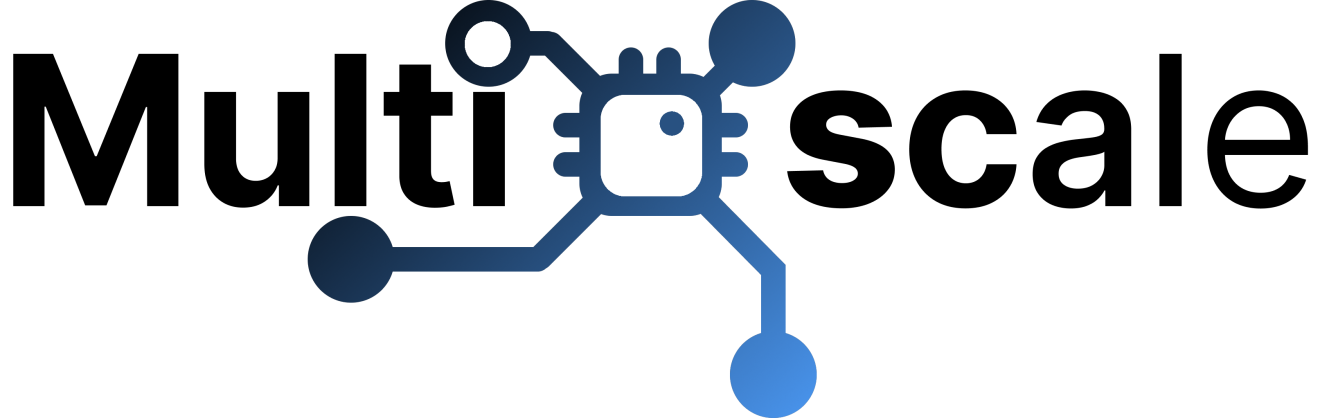
\includegraphics[width=4cm]{multixscale_logo.png}
  \end{center}
\end{columns}
\end{frame}

\placelogofalse
\begin{frame}{waLBerla}
\begin{columns}
\column{0.48\linewidth}
\begin{outline}
  \1 waLBerla framework 
  \2 Introduced in \cite{Bauer2021} (2021)
  \2 HPC-scale simulations
  \2 Stencil problems specifically
  \2 Bring your Compute Kernels
  \1 Provides:
  \2 Multi-node domain partitioning
  \2 Communication patterns 
  \2 Checkpoints
\end{outline}
\column{0.48\linewidth}
\begin{center}
  \shadowimage[width=0.8\linewidth]{juwels.png}
  \vspace{0.5cm}
  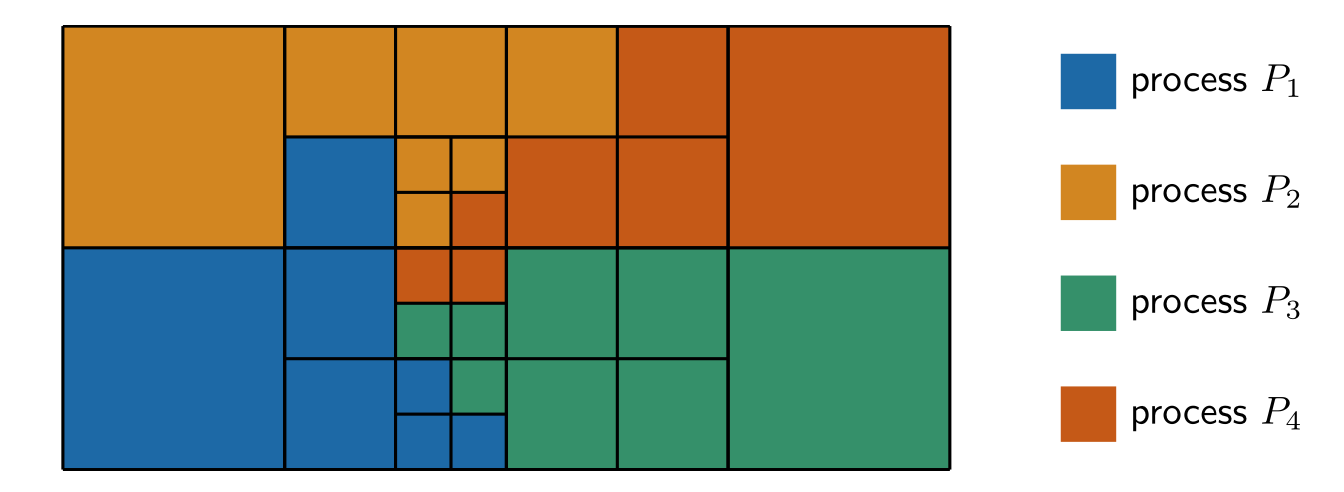
\includegraphics[width=0.8\linewidth]{walberla_partition.png}
  \vspace{0.5cm}
  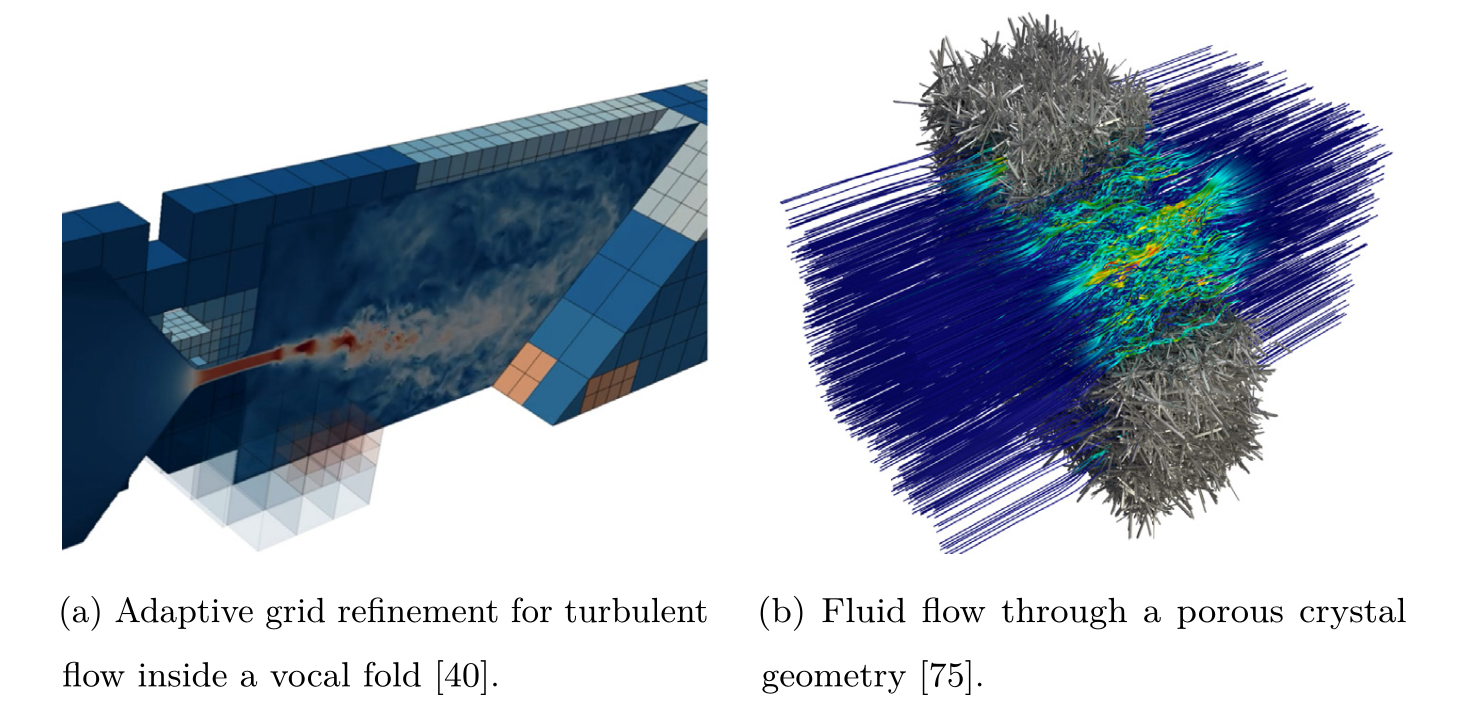
\includegraphics[width=0.8\linewidth]{walberla_examples.png}
\end{center} 
\end{columns}
\blfootnote{From \href{t}{TODO}, \cite{Bauer2021}}
\end{frame}
\placelogotrue


\begin{frame}{\lstinline{pystencils}}
\begin{columns}
  \column{0.48\linewidth}
  \begin{outline}
  \1 Introduced in 2019 \cite{Bauer2019}
  \1 Stencil Compiler 
  \2 \lstinline{sympy}

  \2 Generates optimized compute Kernels
  \2 Introduced in \cite{Bauer2021} (2020)
  \end{outline}

  \column{0.48\linewidth}
  \centering
  \begin{center}
    
\includegraphics[width=0.2\linewidth]{pystencils_logo.png}
  \end{center}
\end{columns}
\end{frame}

\begin{frame}{\lstinline{lbmpy}}
  \begin{columns}
  \column{0.48\linewidth}
  \begin{outline}
  \1 Python package for LBM
  \2 Introduced in \cite{Bauer2021} (2020)
  \end{outline}

  \column{0.48\linewidth}
  \centering
  \begin{center}
    
\includegraphics[width=0.2\linewidth]{lbmpy_logo.png}
  \end{center}
\end{columns}
\end{frame}


% Paper intro
\placelogofalse
\begin{frame}{Introduction}
\begin{columns}
\column{0.48\linewidth}
\begin{outline}
  \1 Presenting \cite{Hennig2023} (2023)
  \2 Adds multiple MRT methods to \lstinline{lbmpy}
  \2 Supports ``arbitrary'' governing eqns
\end{outline}
\column{0.48\linewidth}
\begin{center}
  \shadowimage[width=0.5\linewidth]{hennig_paper.png}

  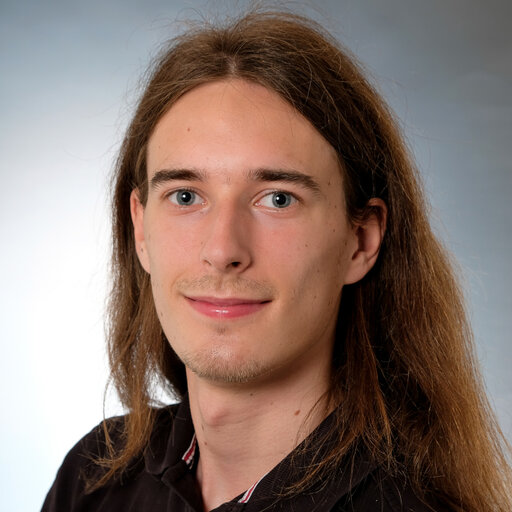
\includegraphics[width=0.3\linewidth]{frederik_hennig.jpg}
  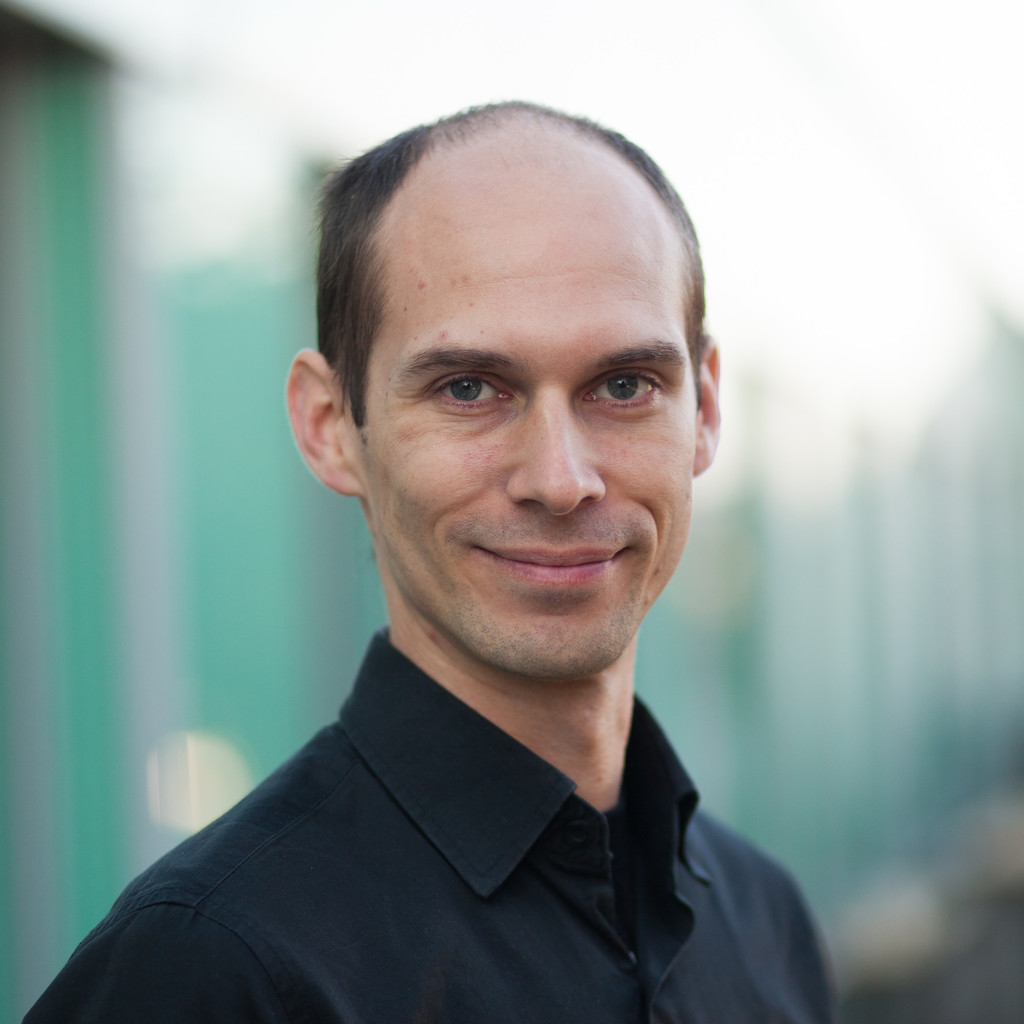
\includegraphics[width=0.3\linewidth]{markus_holzer.jpg}

  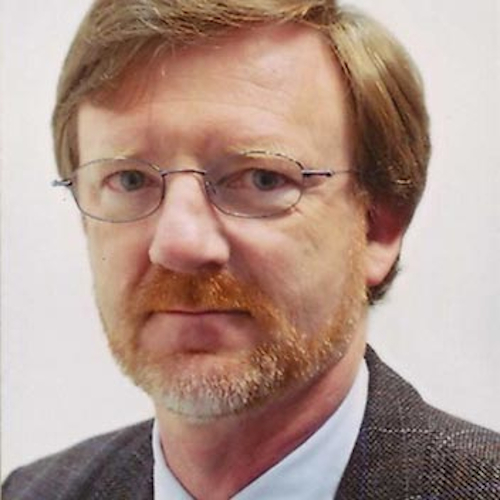
\includegraphics[width=0.3\linewidth]{ulrich_rude.jpg}
\end{center} 
\end{columns}
\end{frame}
\placelogotrue



% Zero-centered
\begin{frame}{Zero-centered Storage}
TODO
\end{frame}


% TODO Simplication Passes 
\begin{frame}{Simplification Passes}
TODO
\end{frame}

\placelogofalse
\begin{frame}{Moments}
\begin{columns}
\column{0.48\linewidth}
\begin{center}
\begin{outline}
\1 Capture integral properties of mass density field
\2 Project onto polynomial basis, $b_i$
\end{outline}
\end{center}

\column{0.48\linewidth}
\begin{center}
  \textbf{Moment}
  $$
  M_{i,j,k} = \int_{\Omega} x^i y^j z^k \rho d\Omega
  $$
  Where $i, j, k \in \{0, 1, 2, \cdots\}$

  \vspace{1.5cm}

  \textbf{Moment Vector}
  \begin{align*}
    \bf{M} &= [M_{0,0,0}, M_{1, 0, 0},\\
      & \cdots, M_{n, 0, 0}, M_{n, 1, 0},\\
      & \cdots, M_{n, n, 0}, M_{n, n, 1},\\
      & \cdots, M_{n,n,n}]^T
  \end{align*}
\end{center}
\end{columns}
\end{frame}
\placelogotrue

\begin{frame}{Quadrature From Moments}
We can approximate an integrand f with weighted basis functions.
$$
f \approx \sum_{i = 1}^n c_i b_i
$$
Then by linearity of integrals
$$
\int_{\Omega} f d\Omega \approx \int_{\Omega} \sum_{i = 1}^n c_i b_i \ d \Omega
= \sum_{i=1}^n c_i \int_{\Omega} b_i \ d \Omega
$$
Where $m_i = \int_{\Omega} f_i d \Omega$
\end{frame}

\begin{frame}{Moment Fitting for Quadrature Rules}
\centering
\begin{center}
$$
\bf{A} \cdot \bf{W} = \bf{M}
$$
Where
$$
\bf{A} = \left[
\begin{array}{cccc}
  b_1(x_1) & b_1(x_2) & \cdots & b_1(x_q) \\
  b_2(x_1) & b_2(x_2) & \cdots & b_2(x_q) \\
  \vdots & \vdots & \ddots & \vdots \\
  b_n(x_1) & b_n(x_2) & \cdots & b_n(x_q) \\
\end{array}\right],
W = \left[
  \begin{array}{c}
    w_1 \\ w_2 \\ \vdots \\ w_q
  \end{array}
\right],
M = \left[
  \begin{array}{c}
    m_1 \\ m_2 \\ \vdots \\ m_q
  \end{array}
\right],
$$
With $m_i = \int_{\Omega} b_i \ d\Omega$
\end{center}
\end{frame}

\begin{frame}{Compress Quadrature}
  \centering
  \begin{center}
    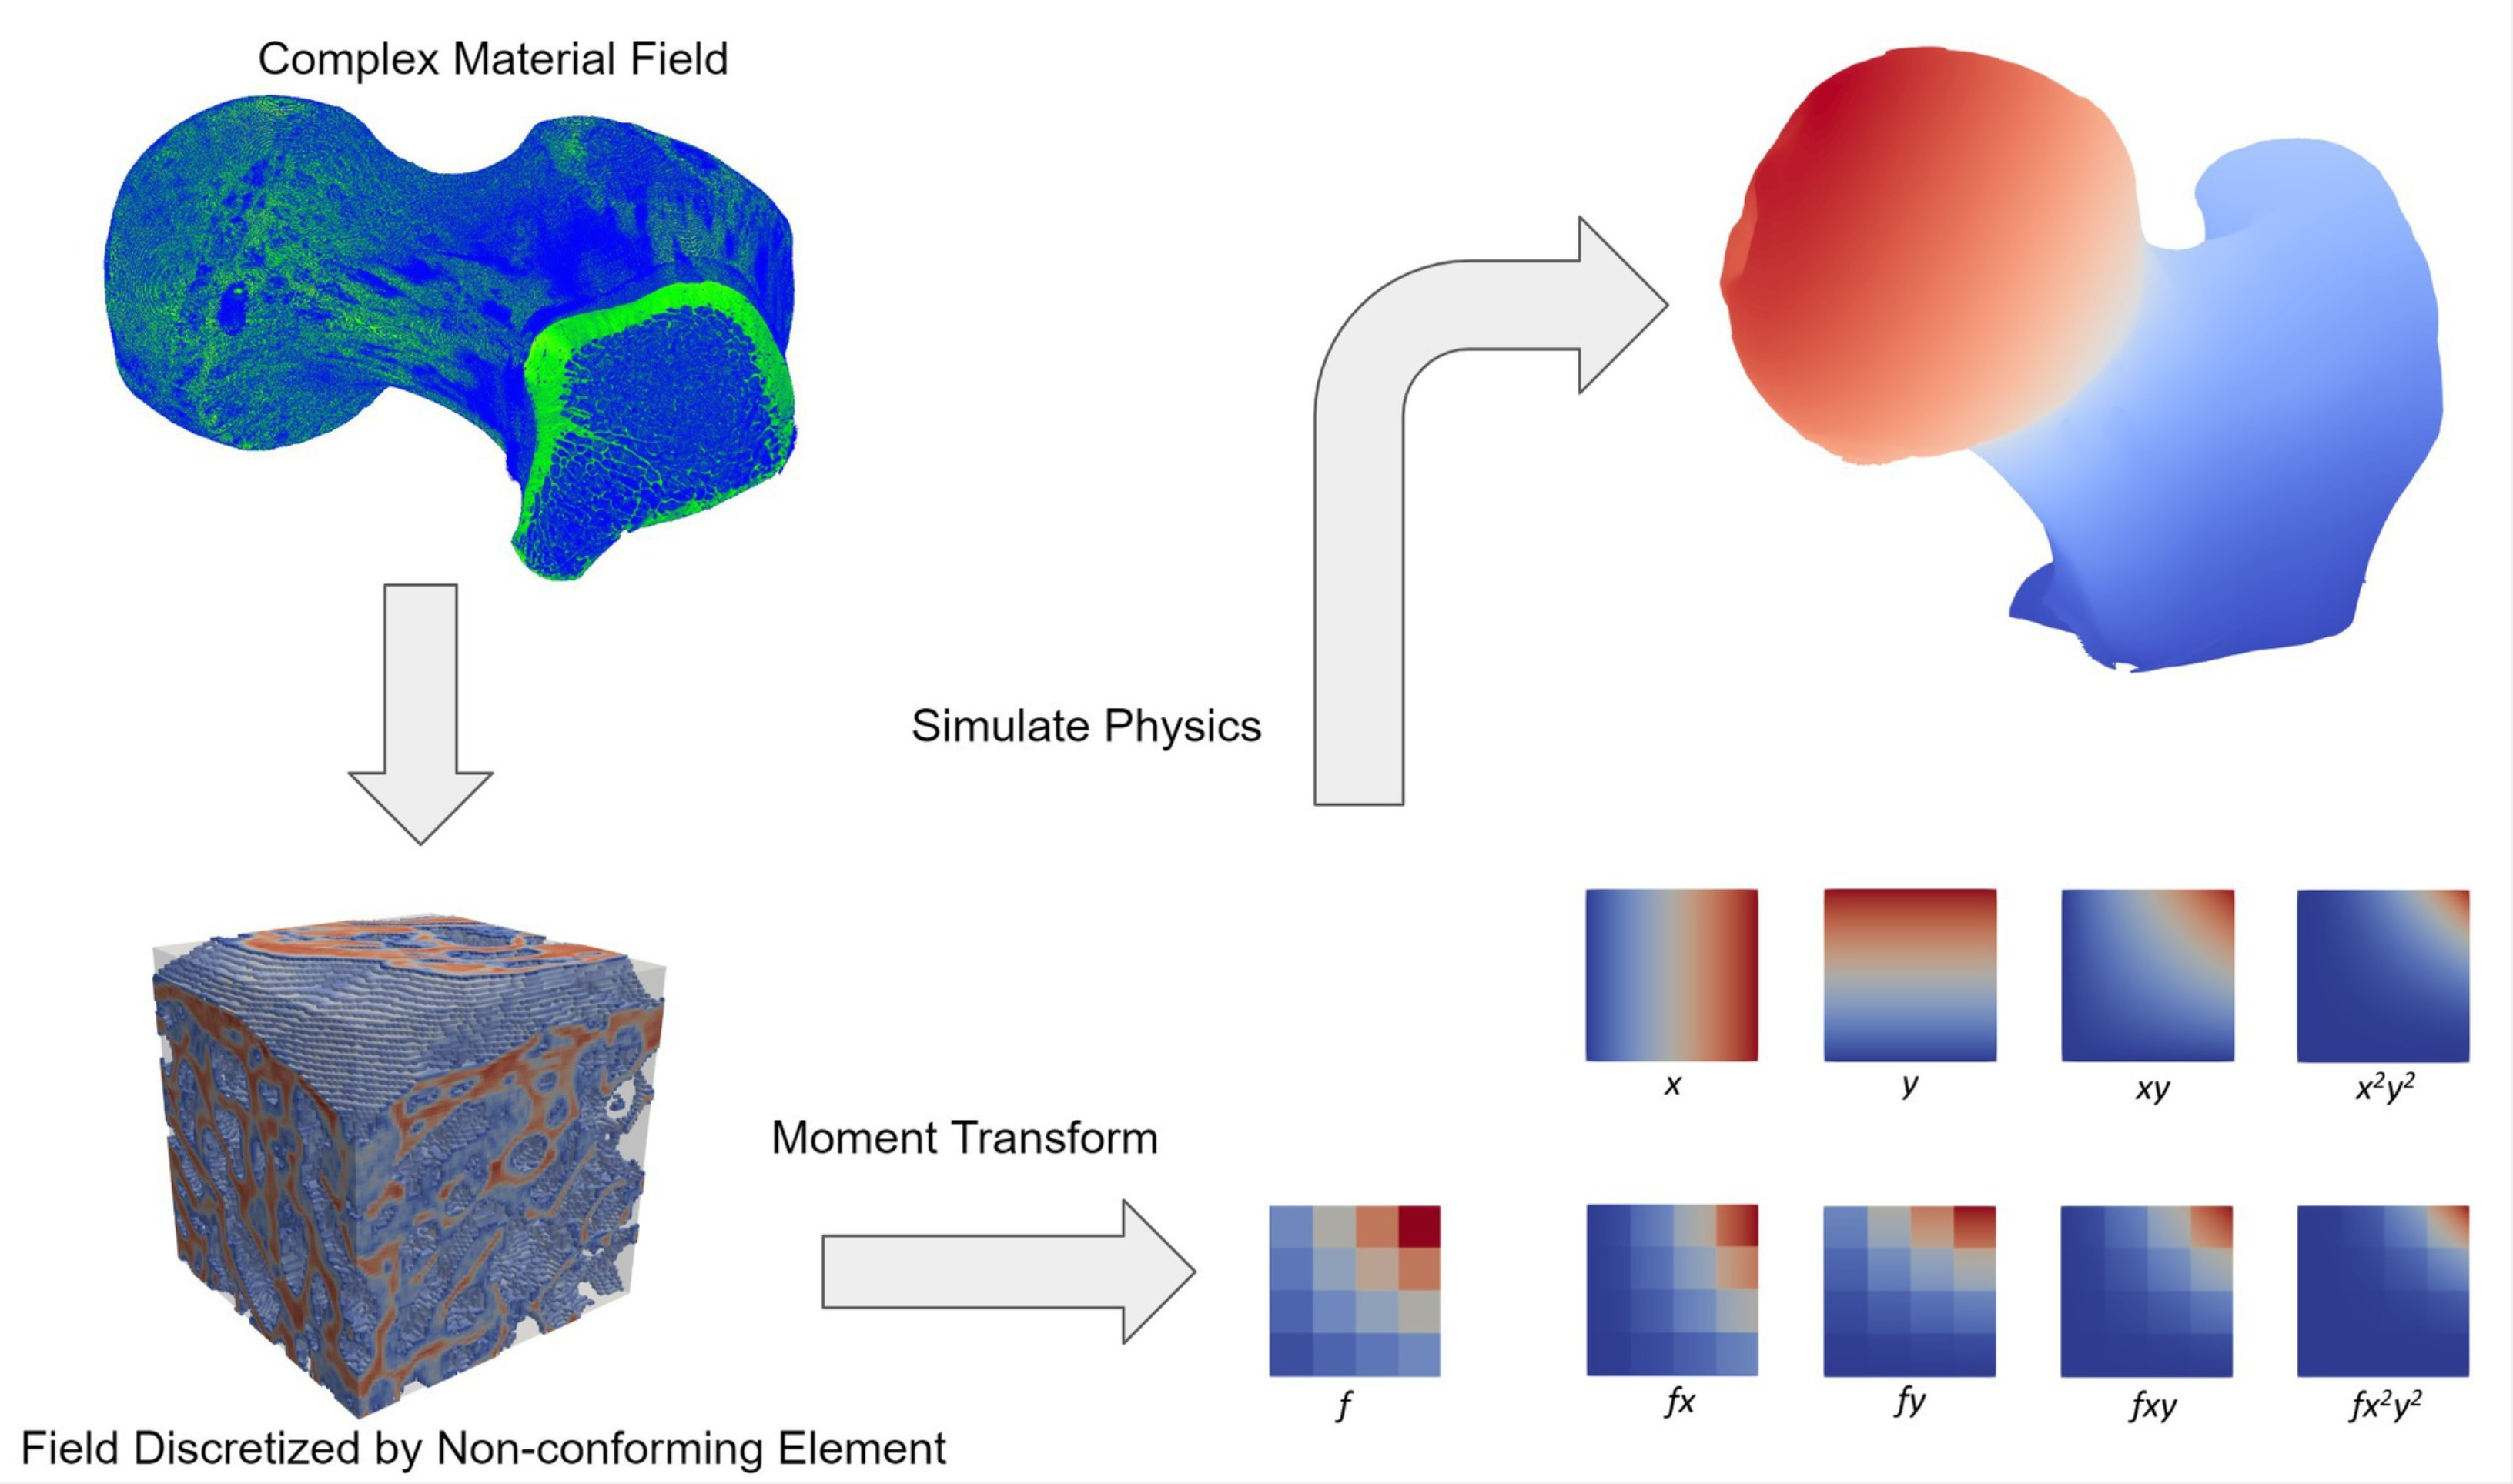
\includegraphics[width=0.8\linewidth]{bone_scan_example.png}\\
  \end{center}
    \blfootnote{Image from \cite{Taber2018}}
\end{frame}

\begin{frame}{Using the Divergence Theorem}
  \begin{center}
    \shadowimage[width=0.6\linewidth]{GeometryCell_scene_1.png}

    \shadowimage[width=0.3\linewidth]{GeometryCell_whole_1.png}
    \shadowimage[width=0.3\linewidth]{GeometryCell_outline_1.png}
  \end{center}
\end{frame}


\begin{frame}{Consequences}
\begin{columns}
\column{0.58\linewidth}
  \begin{outline}
    \1 Generalizes from just density to other fields like conductivity or even stiffness (spatially variable materials)
    \1 This was my job, shuttling data where it needs to be
  \end{outline}
\column{0.38\linewidth}
\begin{center}
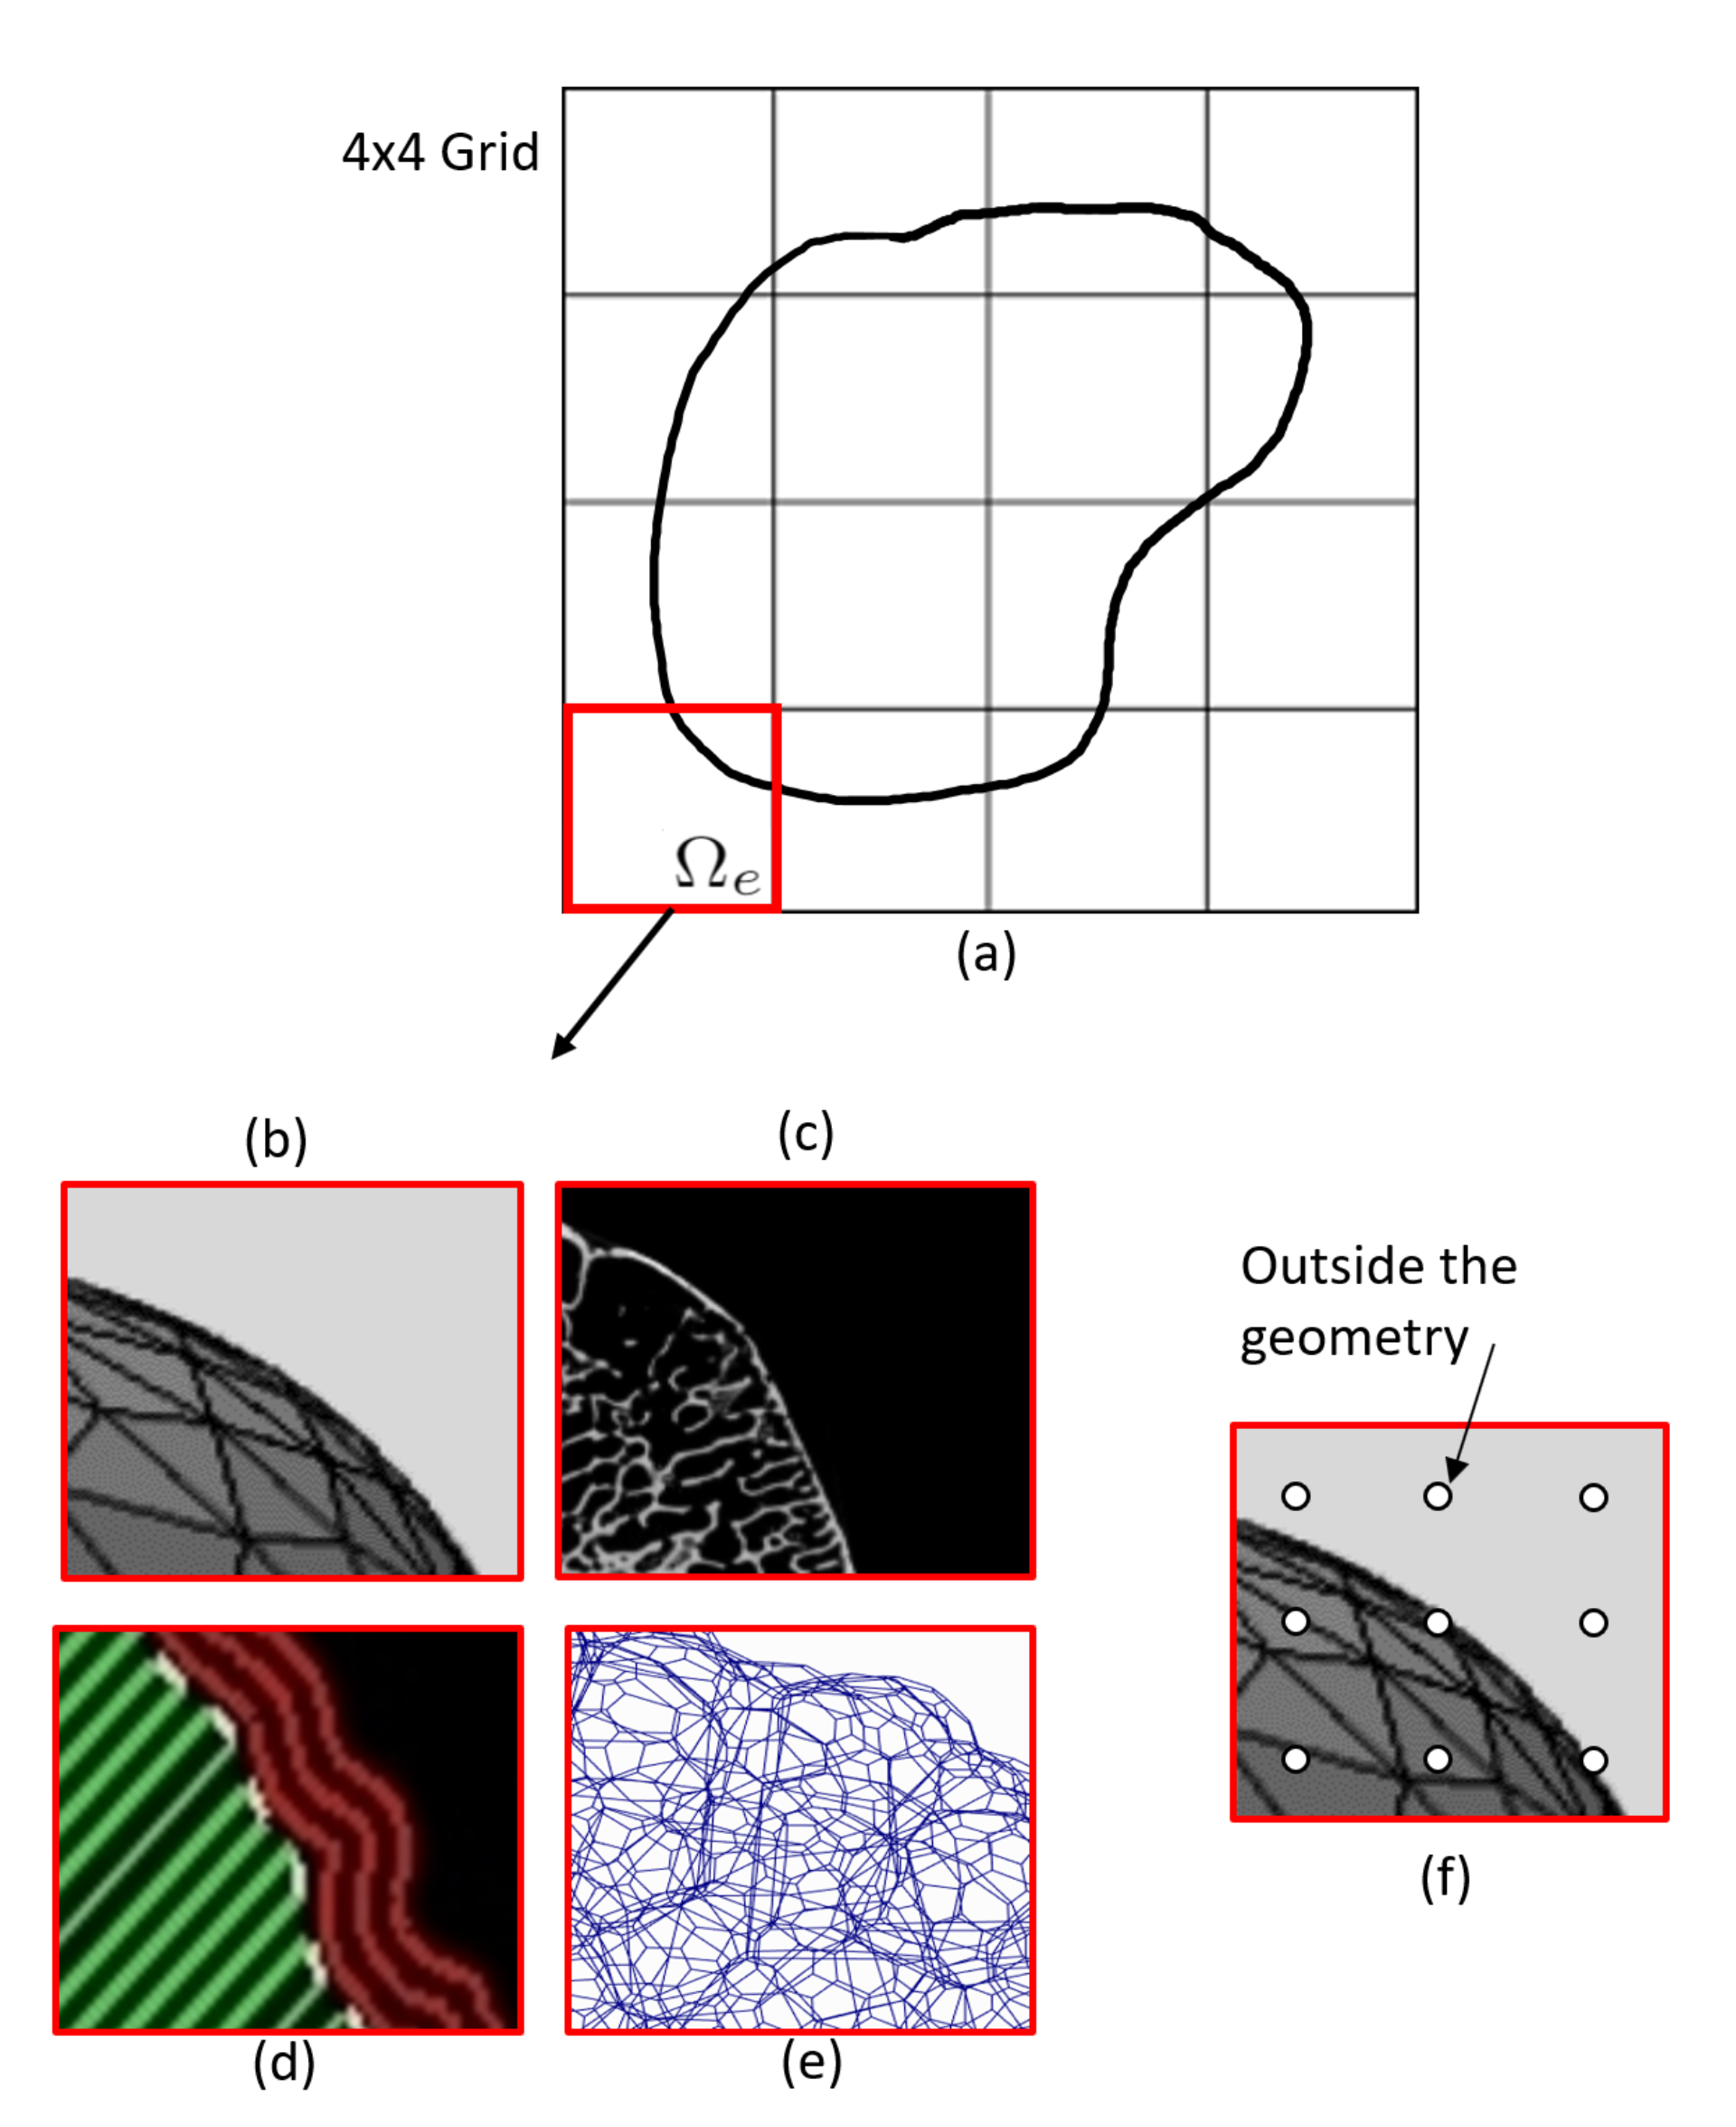
\includegraphics[width=4cm]{immersed_moments.png} 
\end{center}
\end{columns}
\blfootnote{Image from \cite{Taber2018}}
\end{frame}


% "Operation Count"
% rg '\+|\*|\-' cm_lbm_generated/src/shader_ops/cm_mrt.rs -o  | wc -l
\begin{frame}{Symbolic Simplification Results}
  \centering
  \begin{center}
    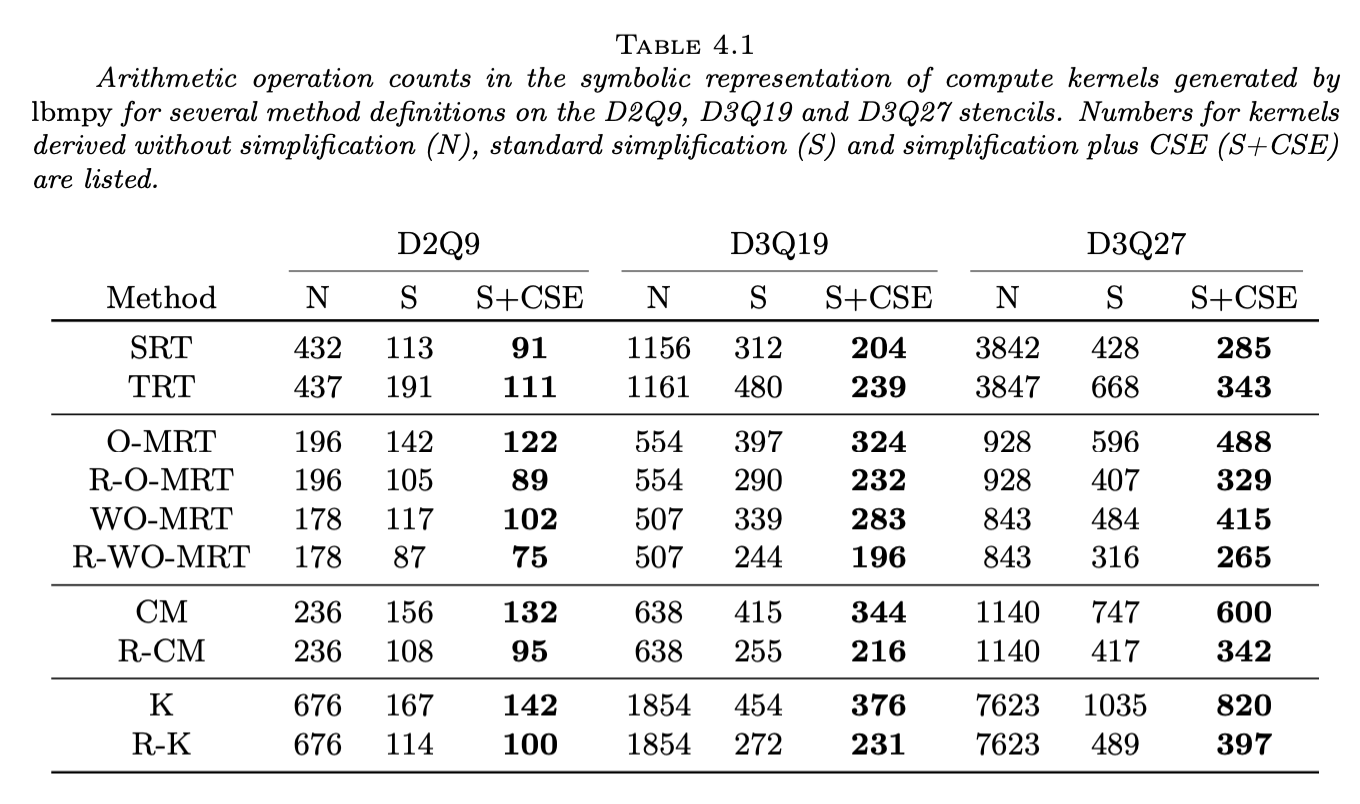
\includegraphics[width=0.8\linewidth]{arith_table.png}
  \end{center}
  For reference, my had \textsc{CM} implementation (slight over estimate) $220,702$ arithmetic operations.
  \blfootnote{From \cite{Hennig2023}}
\end{frame}






% Eh
% \begin{frame}
  \begin{outline}
   \1 \cite{Yu2025Filter}
  \end{outline}
\end{frame}


\begin{frame}[allowframebreaks]{References}
    \tiny
    \printbibliography
\end{frame}

\end{document}


